
\section{Diseño de la arquitectura}

\subsection{Cola de mensajes}
 
El mecanismo de comunicación que se utilizó para el pasaje de información entre
los distintos procesos dentro del trabajo práctico fue, únicamente, la cola de mensages. La 
principal razón por la cual se optó por este mecanismo se debió a que el sincronismo
entre los mensajes escritos y leídos está a cargo del sistema operativo. \\

En un principio se consideró el uso de memoria compartida, sincronizando el acceso a la misma
con semáforos. Esta solución era un poco limitada, ya que acotaba el tamaño de los
datos compartidos a un máximo pre-establecido. En el caso de la tabla de contactos 
se limitaría la cantidad de usuarios registrados y también cuando dos usuarios estuvieran chateando
no podrían enviarse mensajes más extensos que el tamaño de la memoria compartida. 

Por otro lado, se analizó la posibilidad de utilizar tuberías con nombre ya que permitían enviar mensajes
de cualquier longitud. El problema en el uso de fifos estaba relacionado con el sincronismo,
ya que es inaceptable que más de un proceso escriba en forma simultánea en la tubería. Implementar un protocolo sincronizado para las fifos hubiese sido en definitiva hacer \emph{a mano} la cola de mensajes.

Luego de analizar las diferentes alternativas, se optó por utilizar cola de mensajes
ya que era el mecanismo de conumicación que mejor se adaptaba al problema.

\subsubsection*{Mensajes de tamaño variable}

Si bien las colas de mensajes permiten el envío de mensajes de tamaño variable, la implementación de esto no es presisamente directa. \\

La función del sistema \verb|msgsnd| recibe un puntero a un buffer y un tamaño, en bytes, de los datos a enviar. Esto permite, fácilmente, tener control sobre la cantidad de bytes enviados. Sin embargo, para recibir un mensaje es necesario conocer previamente la cantidad de bytes a leer. Por ende, no es posible saber de qué tamaño crear el buffer de lectura que se le pasa a \verb|msgrcv|. \\

Esto se podría solucionar enviando dos mensajes: primero el tamaño en bytes y luego los datos del mensaje en sí. De esa forma, al leer un mensaje primero se recibiría el tamaño (que es un entero que ocupa una cantidad de bytes fijos, por ejemplo 4), y luego, con ese tamaño, leer los datos. Pero esto crea un problema de sincronismo: no se puede asegurar que entre que se envía el primero y el segundo mensajes otro proceso no mande un mensaje a la cola, rompiendo el protocolo. \\

Por fortuna, \verb|msgrcv| informa cuando un mensaje a leer sobrepasa el tamaño del buffer de lectura: retornando -1 y seteando la variable global \verb|errno| a un simpático valor \verb|E2BIG|. De esta forma, se puede hacer un sencillo algoritmo para recibir mensajes de tamaño variable:

\begin{small}
\begin{verbatim}
void* mensaje;
int tamanio_mensaje;

int tamanio_buffer = TAMANIO_BUFFER_INICIAL;
bool mensaje_recibido = false;
while (!mensaje_recibido)
{
    void* buffer = new char[tamanio_buffer];
    int bytes_leidos = msgrcv(id_cola, buffer, tamanio_buffer, mtype);
    if (bytes_leidos == -1 && errno == E2BIG)
    {
        // No alcanzó el tamaño del buffer, re redimensiona.
        delete [] buffer;
        tamanio_buffer *= 2;
    }
    else if (bytes_leidos != -1) 
    {
        // El mensaje entró en el buffer.
        mensaje = buffer;
        tamanio_mensaje = bytes_leidos;
        mensaje_leido = true;
    }
    else {
        // Ocurrió algún error...
    }
}
\end{verbatim}
\end{small}

En escencia, lo que se hace es intentar leer el mensaje con un buffer de un tamaño inicial fijo y, si falla porque el buffer era muy chico, volver a intentar con un buffer del doble de tamaño, y así iterativamente hasta poder leer todo el mensaje. Al final del algoritmo, el puntero \verb|mensaje| queda apuntando al mensaje leido, y \verb|tamanio_mensaje| es el tamaño del mensaje leido. El código utilizado en la aplicación, si bien análogo, no es idéntico a este, ya que se usaron clases y funciones auxiliares, así como tratamiento de los errores con excepciones. \\

\subsection{Arquitectura General}

\subsubsection{Esquema de direcciones}

Cada módulo en ejecución, ya sea el programa de chat (cliente) o el servicio de localización (servidor) tiene asociada una dirección, que se utiliza para que otros módulos en ejecución puedan contactarlo. La dirección de un módulo en ejecución es simplemente su identificador de proceso (pid). \\

\subsubsection{Comunicación entre módulos}

Para recibir mensajes, cada módulo en ejecución controla una cola de mensajes, esto es: sólo él lee mensajes de la cola (pero más de uno puede escribir mensajes en ella). En el caso del servicio de localización, al poder haber a lo sumo uno en ejución en cualquier momento, la cola de mensajes se encuentra en un archivo de dirección fija (configurable a través de un archivo de configuración). En el caso de los clientes que, obiamente, pueden haber muchos en ejecución simultaneamente, su cola está asociada a un archivo con nombre tipo \emph{cliente$<$direccion$>$.queue}, de manera que sea única y sólo un cliente lea de ella.

\subsubsection{División en procesos}

Para el servicio de localización se optó por la solución más sencilla: un único proceso. Dicho proceso es un ciclo infinito que en cada iteración se bloquea hasta recibir un mensaje de su cola de entrada y luego lo procesa. \\

El módulo cliente está dividido en dos procesos: uno muy sencillo encargado de la lectura de teclado y otro que maneja la lógica del cliente (el proceso proncipal). Al leer algun input del usuario por teclado, el proceso de entrada, para informarme al proceso principal de ese evento, le envía un mensaje con contenido del input a través de la cola de mensajes asociada a ese cliente. El proceso principal, análogamente al proceso del servidor, lee mensajes de la cola de entrada y los procesa. Estos mensajes pueden llegar tanto del servidor (como una respuesta de registro de nombre), de un peer (como un mensaje de chat), o del mismo módulo cliente (los mensajes de input desde el proceso de entrada).

%\subsubsection{Cliente-Cliente}
\begin{center}
\small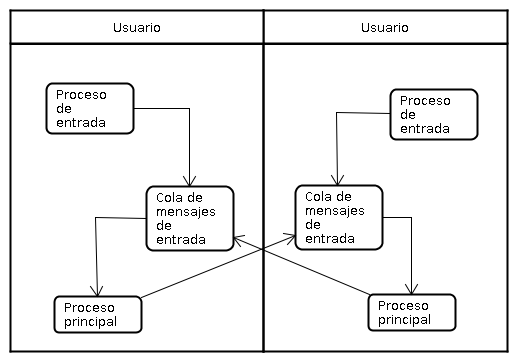
\includegraphics[scale=0.65]{./Images/ArquitecturaClienteConCliente} \\ 
\caption{Equema de comunicación Cliente-Cliente (peer to peer). Las flechas representan entrada y salida de datos. }
\end{center}

%\subsubsection{Cliente-Servicio de localización}
\begin{center}
\small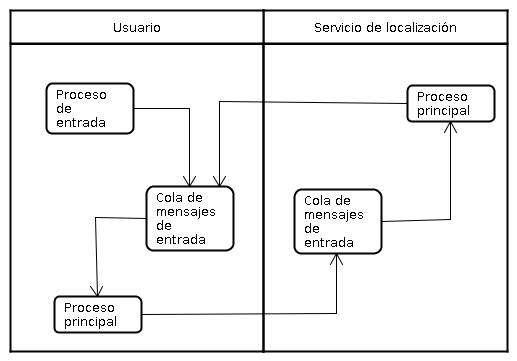
\includegraphics[scale=0.65]{./Images/ArquitecturaClienteConServidor} \\
\caption{Equema de comunicación Cliente-Servicio de localización.} 
\end{center}

\subsection{Diagrama de clases}
\begin{center}
\small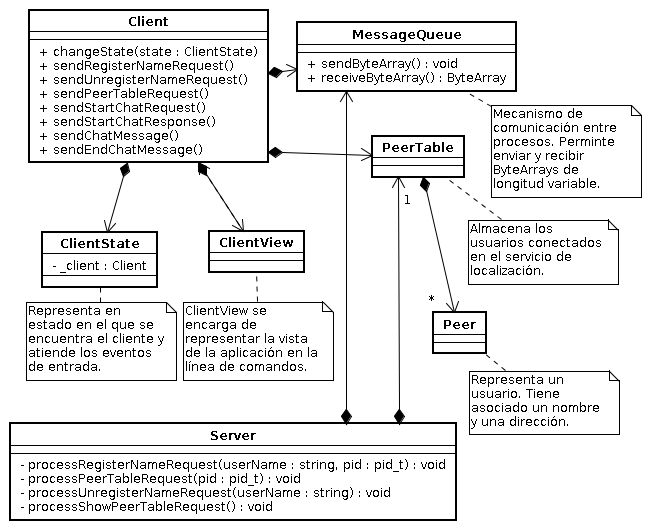
\includegraphics[scale=0.65]{./Images/DiagramaDeClases}
\end{center}

\subsection{Mensajes}

Los procesos se comunican entre sí enviandose mensajes. Se creó una entidad 
llamada ``Message'' la cual encapsula un tipo de mensaje, el id del proceso
creador y los datos asociados el mensaje. Dicho mensaje puede ser serializado
y deserializado para permitir su envio y recepción a través de la cola de mensajes.

\subsubsection{Tipos de mensajes}
\begin{itemize}
  \item {\bf TYPE NONE:} tipo de mensaje inválido.
  \item {\bf TYPE USER INPUT:} enviado desde el proceso que recibe los eventos de teclado \\
hacia el proceso principal cuando el usuario ingresa un comando.
  \item {\bf TYPE USER EXIT:} enviado desde el proceso que recibe los eventos de teclado \\
hacia el proceso principal cuando el usuario ingresa el comando de salida.
  \item {\bf TYPE REGISTER NAME REQUEST:} enviado al servicio de localización para registrar un nuevo usuario.
  \item {\bf TYPE REGISTER NAME RESPONSE:} enviado desde el servicio de localización al usuario para informar \\
si el nombre pudo ser registrado con éxito o no.
  \item {\bf TYPE UNREGISTER NAME REQUEST:} enviado al servicio de localización para desregistrar un usuario.
  \item {\bf TYPE SHOW PEER TABLE REQUEST:} enviado al servicio de localización para hacer que muestre la \\
tabla de contactos.
  \item {\bf TYPE PEER TABLE REQUEST:} enviado al servicio de localización por parte de un usuario para solicitar \\
la tabla de contactos actual.
  \item {\bf TYPE PEER TABLE RESPONSE:} enviado desde el servicio de localización al usuario como respuesta \\
de la solicitud de la tabla de contactos. 
  \item {\bf TYPE START CHAT REQUEST:} enviado entre usuarios para solicitar el comienzo de una seción de chat.
  \item {\bf TYPE START CHAT RESPONSE:} enviado entre usuarios para confirmar o rechazar el inicio de la seción de chat.
  \item {\bf TYPE END CHAT:} enviado entre usuarios para informar el fin de la seción de chat.
  \item {\bf TYPE CHAT MESSAGE:} enviado entre usuarios. Mensaje de chat.
  \item {\bf TYPE SERVER EXIT:} enviado al servicio de localización para cerrarlo remotamente.
\end{itemize}

\subsection{Estados del cliente}

El cliente atiende ditintos tipos de eventos: mensajes de entrada del usuario, mensajes desde otros peers, mensajes desde el servidor. El significado de estos eventos depende del estado en el que se encuentre la aplicación al momento de recibirlos. 

Por ejemplo, si dos usuarios se encuentran chateando, y uno usuario ingresa un comando 
``-usuarios'' (visualizar la tabla de contactos concetados) se esperaría que el usuario con el que se encuentra
chateando reciba un mensaje en texto plano con el contenido ``-usuarios'' y no que visualice la
tabla de contactos en su terminal (lo cual ocurriría si todavía no se está chateando con otro peer). Por esta razón, se optó por el uso del patrón de diseño ``State'' (o estado) el cual nos permite modelar los ditintos estados del cliente en clases separadas y que la clase Cliente le delegue el procesamiento de los distitintos tipos de mensaje a su estado actual.  

\subsubsection{Diagrama de estados}
\begin{center}
\small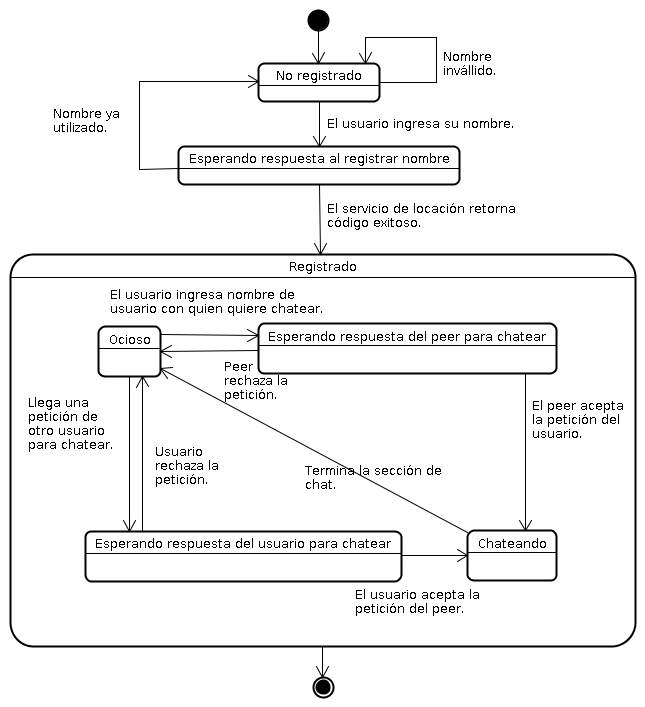
\includegraphics[scale=0.65]{./Images/DiagramaDeEstados}
\end{center}

\subsubsection{Diagrama de clases de los estados}
\begin{center}
\small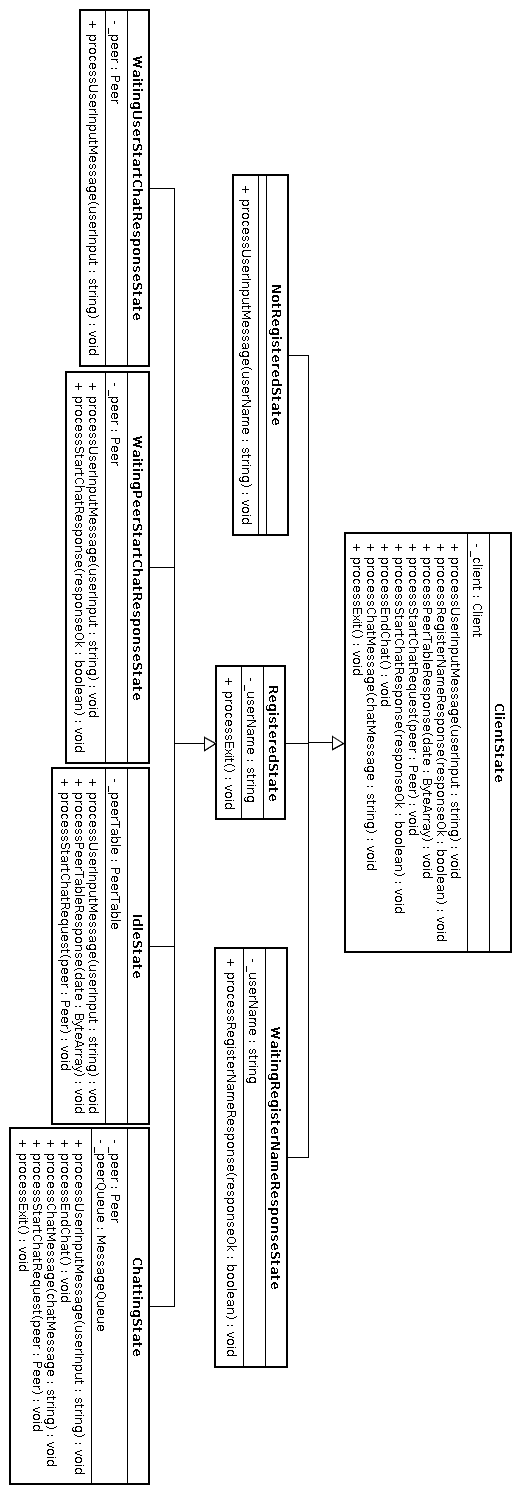
\includegraphics[scale=0.45]{./Images/DiagramaDeClasesDeLosEstados2}
\end{center}

